\documentclass[a4paper,11pt,exos]{nsi} % COMPILE WITH DRAFT
\usepackage{pifont}
\usepackage{fontawesome5}
\usepackage{hyperref}



\begin{document}
\classe{\premiere spé}
\titre{Exo 2 - Probabilités conditionnelles}
\maketitle

\subsection*{Formule des probabilités totales}
\exo{}
Un piéton arrive à un passage protégé. D'après une étude statistique, on établit que le feu piéton est vert avec une probabilité de 0,45. Si le feu est vert, alors le piéton s'engage sur le passage avec une probabilité de 0,9. Sinon, il s'engage avec une probabilité de 0,3.
\begin{enumerate}
    \item Représenter cette situation par un arbre de probabilité et le compléter entièrement.
    \item Calculer la probabilité que le piéton s'engage sur le passage protégé.
\end{enumerate}


\exo{}
L'arbre ci-dessous modélise une expérience aléatoire et quatre événements $A,B, C$ et $D$.\\
\dleft{11.5cm}{
    \begin{enumerate}
        \item Compléter le tableau ci-dessous puis en déduire $P(A)$.
        \begin{center}
            \tabstyle[UGLiOrange]
            \begin{tabular}{|c|c|c|c|c|}
            \hline
            \bcell &\ccell $B$ & \ccell $C$ & \ccell $D$ & \ccell Total \\\hline
            \ccell $A$ & $\qquad$ & $\qquad$ & $\qquad$ & $\qquad$ \\\hline
            \ccell $\overline{A} $ & & & & \\\hline
            \ccell Total  & & & & \\\hline
            \end{tabular}
        \end{center}
        \item Retrouver ce résultat sans utiliser le tableau.
    \end{enumerate}
}{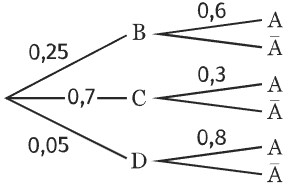
\includegraphics[width=5cm]{arbre1.jpg}}

\exo{}
\dleft{11.5cm}{
    On considère trois événements $A,B$ et $C$ qui forme une partition de l'univers $\Omega$ ainsi qu'un événement $E$.\\
    On donne l'arbre de probabilité ci-contre.
    \begin{enumerate}
        \item Compléter cet arbre de probabilité.
        \item Calculer $P(E)$.
    \end{enumerate}
}
{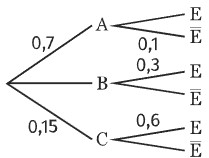
\includegraphics[width=5cm]{arbre2.jpg}}

\exo{}
\dleft{13.3cm}{
    On lance un dé non truqué à six faces numérotées de 1 à 6 et on note le résultat obtenu. Si le résultat est pair, on lance un dé non truqué à 20 faces numérotées de 1 à 20. Si le résultat est impair, on lance un dé non truqué à huit faces numérotées de 1 à 8.
}
{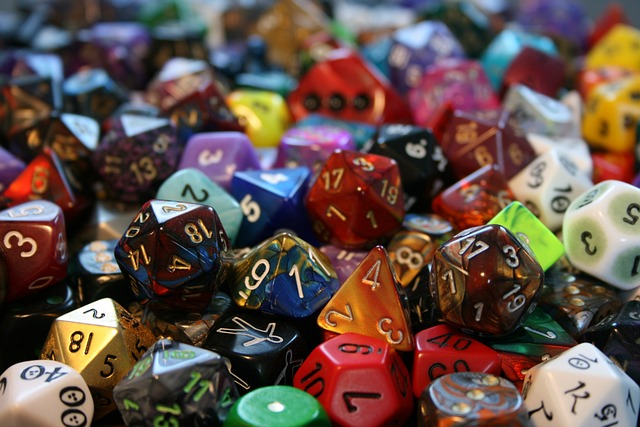
\includegraphics[width=3cm]{dice-568105_640.jpg}}

Quelle est la probabilité pour que le résultat du deuxième dé soit un nombre premier ?


\exo{}
On considère deux événements $A$ et $B$ tels que $\quad P(A)=0,6 \ ; \quad P(B)= 0,4\quad$ et $\quad P_A(B)=0,5$.\\
Calculer $\quad P_{\overline{A}}(B)$.

\exo{}
On jette un dé non truqué à 20 faces numérotées de 1 à 20. On note :
\begin{enumerate}[label=\textbullet]
    \item $A$ : « le résultat est pair » ;
    \item $B$ : « le résultat est l'un des nombres 1 ; 3 ; 5 ; 7 ; 11 ; 13 ; 17 ; 19 » ;
    \item $C$ : « le résultat est impair » ;
    \item $D$ : « le résultat est l'un des nombres 9 ou 15 » ;
    \item $E$ : « le résultat est un nombre premier ».
\end{enumerate}
\begin{enumerate}
    \item $E$ et $A$ forment-ils une partition de l'univers ?
    \item $C$ et $\overline{B}$ forment-ils une partition de l'univers ?
    \item  Parmi ces cinq événements, en donner deux qui forment une partition de l'univers.
    \item Parmi ces cinq événements, en donner trois qui forment une partition de l'univers.
\end{enumerate}

\exo{}
Dans la famille Tuche, la probabilité de manger du gratin un jour donné est égale à 0,3 si on en a mangé la veille, alors qu'elle est égale à 0,8 si on n'en a pas mangé la veille. Le dimanche, la famille Tuche ne mange jamais de gratin.
On notera les événements suivants :
\begin{enumerate}[label=\textbullet]
    \item $L$: « la famille mange du gratin lundi » ;
    \item $M$: « la famille mange du gratin mardi ».
\end{enumerate}
Quelle est la probabilité que la famille Tuche mange du gratin le mardi ?

\exo{}
Une fourmi a découvert une source de nourriture et en marque le chemin à l'aide de phéromones. Ainsi, la fourmi suivante aura une probabilité égale à 0,95 de retrouver le chemin de la source de nourriture. Au bout d'un certain temps, la piste de phéromone disparaît et les fourmis suivantes n'ont plus alors qu'une probabilité égale à 0,1 de trouver la source de nourriture. La probabilité que la deuxième fourmi arrive avant la disparition des phéromones est 0,45.
\begin{enumerate}
    \item Quelle est la probabilité que la seconde fourmi trouve la source de nourriture ?
    \item Si la deuxième fourmi a trouvé la source de nourriture, elle dépose à nouveau des phéromones. Une troisième fourmi cherche la source de nourriture. Elle commence son trajet au moment où les phéromones de la première ont disparu mais où les éventuelles phéromones de la deuxième sont toujours actives.\\
    On ignore si la deuxième fourmi a trouvé la nourriture : calculer alors la probabilité que la troisième fourmi trouve la nourriture.
\end{enumerate}

\exo{}
Lorsqu'elle est exposée au virus de la grippe, une personne peut développer la grippe. Quand elle est vaccinée, la personne exposée ne développe pas la maladie avec une probabilité égale à $\alpha$. $\alpha$ s'appelle l'efficacité du vaccin.\\
De plus, on constate que, parmi les personnes exposées, 20 \% ne sont ni vaccinées, ni malades. Cette année, la probabilité qu'une personne exposée soit vaccinée est égale à 0,4.
\begin{enumerate}
    \item Exprimer, en fonction de $\alpha$, la probabilité qu'une personne exposée soit vaccinée et ne soit pas malade.
    \item Exprimer, en fonction de $\alpha$, la probabilité qu'une personne exposée soit vaccinée et malade.
    \item Pour quelle valeur de α la proportion de personnes exposées qui ne sont pas malades est égale à 50 \% ?
\end{enumerate}


\exo{}
Votre ami vient de passer les tests de dépistage d'une maladie rare et incurable qui touche une personne sur 100 000. Malheureusement, le test est positif. Espérant une erreur de diagnostic, votre ami a demandé quelle était la probabilité d'une erreur : le spécialiste lui a répondu que, pour 99\% des malades, le résultat est positif, alors que, pour 99,9 \% des personnes saines, le résultat est négatif.
De manière surprenante, vous réussissez à utiliser ces données pour remonter le moral de votre ami.
Soient $M$ et $T$ les événements :
\begin{enumerate}[label=\textbullet]
    \item $M$ : « la personne est malade » ;
    \item $T$ : « le test est positif ».
\end{enumerate}
\begin{enumerate}
    \item Déterminer la probabilité qu'une personne choisie ait un test positif.
    \item Déterminer la probabilité qu'une personne soit malade, sachant que le test est positif.
    \item Rassurer votre ami.
\end{enumerate}

\exo{}
Chaque année, une ruche a un risque de 5 \% d'être attaquée par un frelon asiatique. Dans ce cas, ses chances de survie sont de 10 \%. Si la ruche n'est pas attaquée, ses chances de survie sont de 90 \%. Chaque année, le risque d'attaque est le même et les attaques sont indépendantes les unes des autres.
\begin{enumerate}
    \item Quelle est la probabilité que la ruche survive trois ans ?
    \item Quelle serait cette même probabilité si la menace du frelon asiatique n'existait pas ?
\end{enumerate}
\end{document}